\chapter{結論與未來展望}
\section{結論}
\indent
本論文修改了 Linux kernel 之中 LightNVM 模組,調整寫入模式,讓 LightNVM 從原本不管資料的種類,只循序寫入的方式,改成可將熱門資料以及冷門資料分群的方式寫入SSD,最後經實驗驗證的確有讓 Garbage Collection 的次數下降,提升 Garbage Collection 的效率。不過在寫入效能方面是幾乎沒有影響,經我們分析,如果 Garbage Collection 設計得宜,應該是要盡可能地不要妨礙讀取或寫入的任務,所以我們即使提升了 Garbage Collection 的效率,對於提升寫入效能的成效有限是合理結果。

%\indent
%本論文擴充了劉冠志論文\cite{LIU-Thesis}於Eclipse實作之外掛程式RF Refactoring,增加了兩種重構方法,不只讓團隊於選擇重構方法時能夠更加多元,且能夠減少搜尋的缺漏及取代的錯誤。根據第三章RF Refactoring延伸功能之設計,使擴充後的RF Refactoring在搜尋重複步驟時,能夠確實地得到需要進行新關鍵字取代之重複步驟,而不是得到與團隊需求不同之步驟;此外移動關鍵字宣告後,其搜尋原先使用關鍵字之測試腳本時,也能夠確實地得到真正有使用被移動之關鍵字的測試腳本,而不是得到使用類似名稱之關鍵字的測試腳本等等。

%\indent
%第四章中將擴充之重構功能結合至原先已存在之外掛程式RF Refactoring後,使用者不必進行搜尋,即可得知其需要被取代的重複步驟,並且可以依照需求進行選擇,而移動關鍵字宣告後,也不需要自行引入測試腳本所需之測試資源,即可完成重構。由第五章中可得知,當團隊遇到實際案例時的重構過程,並且使用擴充後之RF Refactoring,確實可以減少重構之時間,因而提升整體重構效率,此外,案例中的測試專案規模較小,能夠減少重構的時間也相對較少,如果將擴充後之RF Refactoring應用於規模更加龐大的測試專案,其能夠減少的重構時間也能夠相對上升。
%\newpage

\section{未來方向}
\indent
本論文修改 LightNVM 之設計仍有待改善之處,以下說明:

\begin{itemize}
    \item\textbf{寫入模式之調整:}
    於\ref{s3.3}節的寫入過程,如果可以將 entry 的資料實際寫入所指向的 Line;而不是讓 LightNVM 用原本的挑選模式挑選完之後,將 entry 所指向的 Line 總和平均,再切換 Line。這樣應該可以更加提升效率(如圖\ref{f5.1}所示)。

    %\item\textbf{執行重構之效能:}
    %本論文擴充之測試腳本重構工具在執行任一重構方法前,都必須先行解析測試專案下的所有測試資料,而使用者通常必須花費較長時間等待其解析完成,並且專案中的資料越多時,則等待時間也會相對增加。若能在啟動重構工具時,利用其他執行緒事先於背景解析專案下之測試資料,且資料有任何新增、修改、刪除等操作時,則再次重新解析相對應資料,確保檔案內容之正確,即可消除執行重構方法時的等待時間,使重構效率更加提升。

    %\item\textbf{重構方法之新增:}
    %測試腳本重構工具經本論文擴充後,其重構方法目前有五個,重新命名關鍵字、重新命名變數、修改關鍵字介面、包裹重複步驟成為新關鍵字及移動關鍵宣告,重構方法擁有十分多種,而測試人員於開發時,也會有遭遇其他重構需求的時候,因此如果能夠增加更多種類之重構方法,其能減少測試人員於手動重構時錯誤及缺漏的產生,表\ref{t6.1}為未來可擴充之重構方法。

    %\item\textbf{其他功能:}
    %本論文所擴充之測試腳本重構工具是參考其他IDE重構功能所開發,因此於重構完成後必須手動執行被重構之測試腳本,才可知道其是否測試功能與未重構前相同,若能與其他測試腳本變更偵測工具結合,例如:邱文煜論文\cite{CHIU-Thesis}所提供之測試選擇工具,於重構完成後,即可執行有所變更之測試腳本,能夠更快地知道重構後之結果是否如測試人員所需,縮短測試人員於重構後之確認時間。

\end{itemize}

\begin{figure}[H]
    \centering
    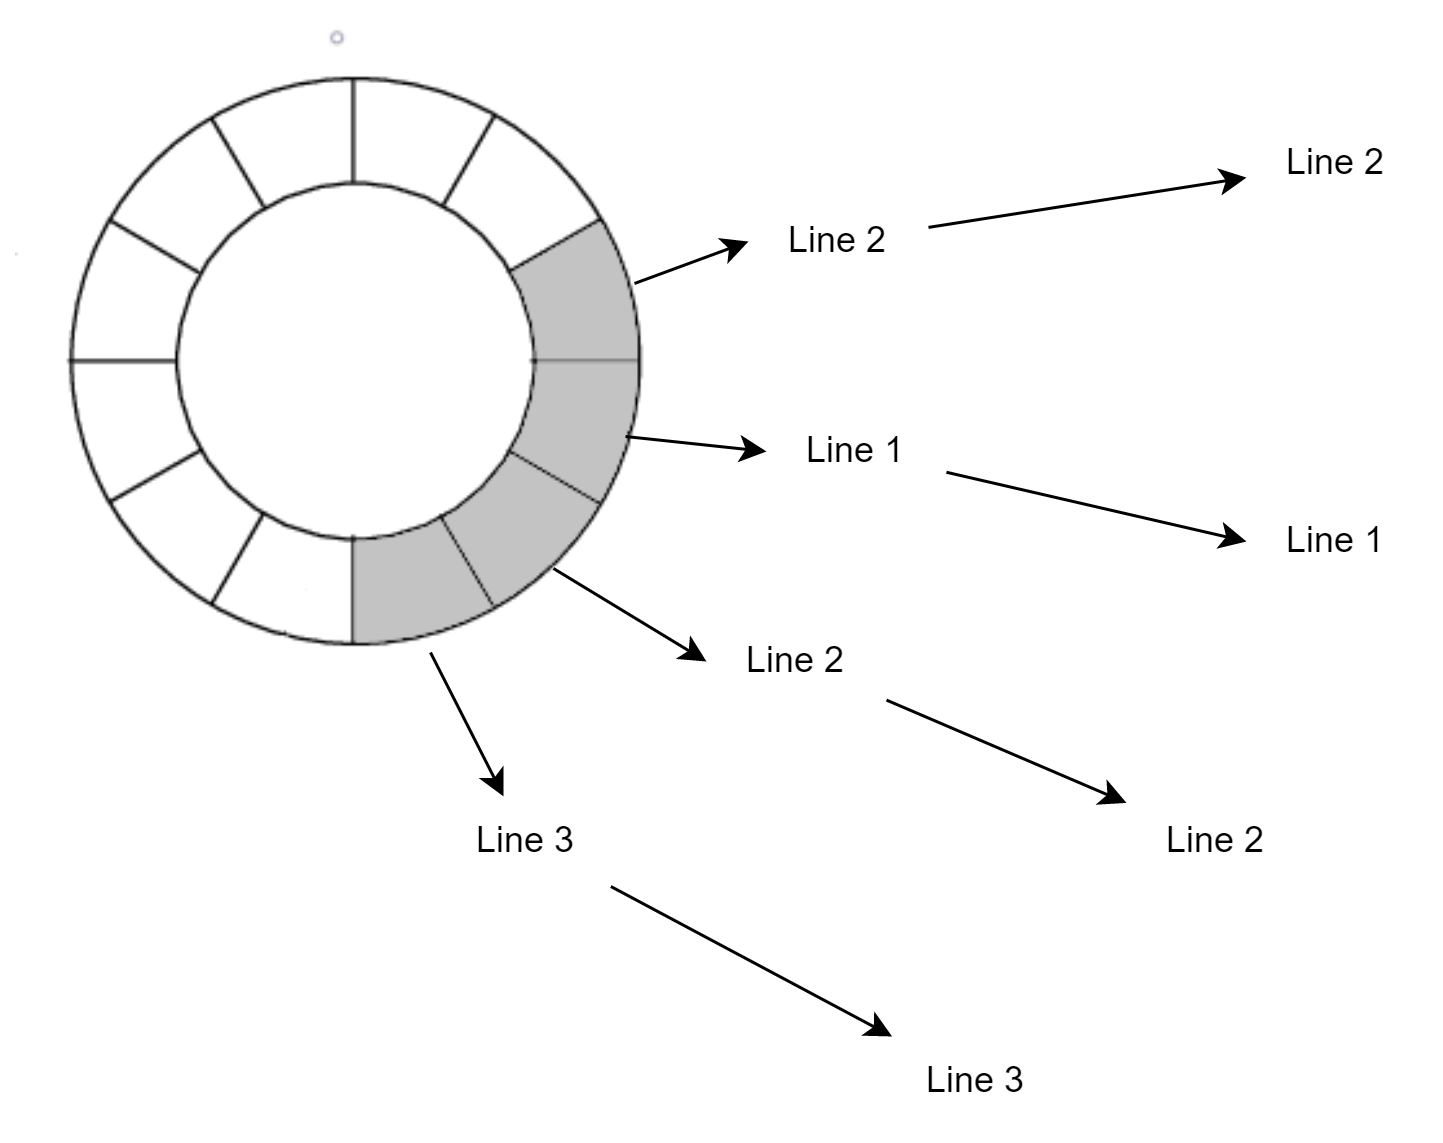
\includegraphics[width=0.8\textwidth]{picture/ch5/future.png}
    \caption{Entry 代表的資料可寫入至對應的 Line}
    \label{f5.1}
\end{figure}